\section{Einführung}
	\subsection{Aufgabenstellung}
	
	\subsubsection{Reaktorstart}
	\begin{itemize}
	\item Zunächst wird durch Abarbeiten des Betriebsschemas eine Funktionskontrolle durchgeführt und protokolliert.
	\item Mittels Wiederholungsstart wird der Reaktor hochgefahren. Dabei soll der kritische Zustand bei P$=\unit[1]{W}$ erreicht werden.
	\item An ausgewählten Messpunkten sind die Gamma- und Neutronendosisleistung bei einer Leistung von $\unit[1]{W}$ und $\unit[2]{W}$ zu messen.
	\item Die entsprechenden Steuerstabsstellungen des kritischen Zustanden bei unterschiedlichen Leistungen werden ermittelt. 
	\end{itemize}
	
	\subsubsection{Steuerstabskalibrierung}
	\begin{itemize}
	\item Das Prinzip der stabilen Reaktorperiode T wird genutzt, um zwei Steuerstäbe mittels Kompensationsmethode in Abhängigkeit der Positionen zu kalibrieren. Über die INHOUR Gleichung werden die dazugehörigen Reaktivitäten berechnet.
	\item Dazu werden jeweils die differentielle und die integrale Steuerstabskennlinie graphisch dargestellt.
	\item Anhand der Kennlinien werden sowohl die Überschussreaktivität als auch die Abschaltreaktivität bei partieller Abschaltung bestimmt.
	\end{itemize}
	
	\subsubsection{Reaktivität einer Cadmiumprobe}
	\begin{itemize}
	\item Durch das Einführen einer Cadmiumprobe in einen der Experimentierkanäle wird unter Zuhilfenahme der Steuerstabskennlinien deren Reaktivität bestimmt.
	\end{itemize}
	
	\subsection{Reaktoraufbau und Sicherheitsmechanismen}
	Der AKR ist ein thermischer, homogener, feststoffmoderierter Nullleistungsreaktor. Er befindet sich im thermischen Gleichgewicht mit der Umgebung. Die weiteren Eigenschaften werden im folgenden erklärt.
	Der schematische Aufbau ist in den Abbildungen \ref{fig: Horizontaler Querschnitt} und \ref{fig: Vertikaler Querschnitt} dargestellt. Die Kettenreaktion wird durch eine $ ^{241} $Americium-Beryllium Neutronenquelle mit einer Aktivität von $\unit[2,2 \cdot 10^{6}] {Bq}$ initialisiert. Sie wird dafür an das untere Ende der zylindrischen Spaltzone gefahren. Diese besitzt einen Durchmesser von $\unit[250]{mm}$ und eine Höhe von $\unit[275]{mm}$. Sie ist im abgeschalteten Zustand aus Sicherheitsgründen in zwei zylindrische Hälften geteilt. Durch den Spalt gehen viele Neutronen für die Kettenreaktion verloren. Die Kernhälften bestehen aus runden Brennstoffplatten eines homogenen Gemisches aus 19,8\% mit Uran-235 angereichertem Uranoxid (Brennstoff) und Polyäthylen (Feststoffmoderator). Die Hälften werden durch einen Aluminiumbehälter hermetisch umschlossen. Zur Regelung der Kettenreaktion thermischer Neutronen dienen die drei Steuerstäbe aus Cadmium, welche separat angesteuert und vertikal bewegt werden können (vgl. Schema in Abb. \ref{fig: Reaktoraufbau}). Dieser Aufbau befindet sich in einem gasdichten Tank, in welchem bezüglich der Umgebung ein Unterdruck herrscht. Dies beugt einem Austreten von Spaltprodukten vor. Der Tank wird schließlich von einem Graphitreflektor umhüllt. Seine Aufgabe ist es, die aus der Spaltzone austretenden Neutronen zurück zu reflektieren und damit die Neutronenflussdichte zu erhöhen.\\
	Zur Abschirmung nach außen dient zum einen eine 12 cm dicke Paraffinschicht. Durch die enthaltenen Wasserstoffatome werden mögliche austretende Neutronen weiter abgebremst. % WW Bild
	Zum anderen ist der Reaktor abschließend durch 480 mm dicken Barytbeton in radiale Richtung und 630 mm in axiale Richtung umgeben. Dieser schirmt entstehende $\gamma$-Strahlung ab.\\
	Für verschiedene Experimente stehen 4 horizontale und zwei vertikale Experimentierkanäle zur Verfügung. Der vertikale als auch horizontale Querschnitt des Reaktors sind jeweils in Abbildung \ref{fig: Vertikaler Querschnitt} und \ref{fig: Horizontaler Querschnitt} zu sehen.
	
	
	
	\begin{figure}[ht]
	\centering
	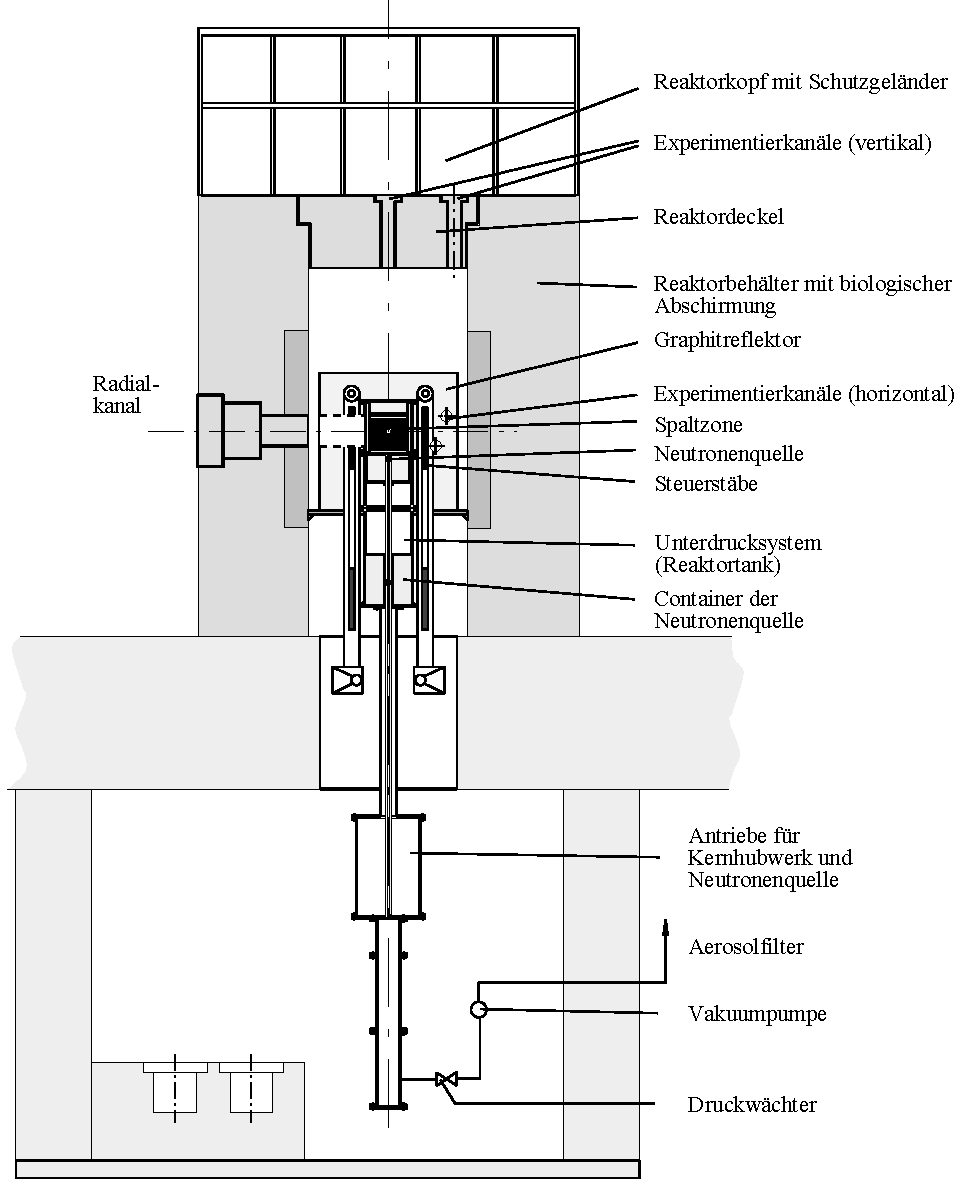
\includegraphics[width=0.7\textwidth]{pic/Vertikalquerschnitt_Reaktor.pdf}
	\caption{Vertikaler Querschnitt, \cite{Aufbau} }
	\label{fig: Vertikaler Querschnitt}
	\end{figure}
	
	\begin{figure}[ht]
	\centering
	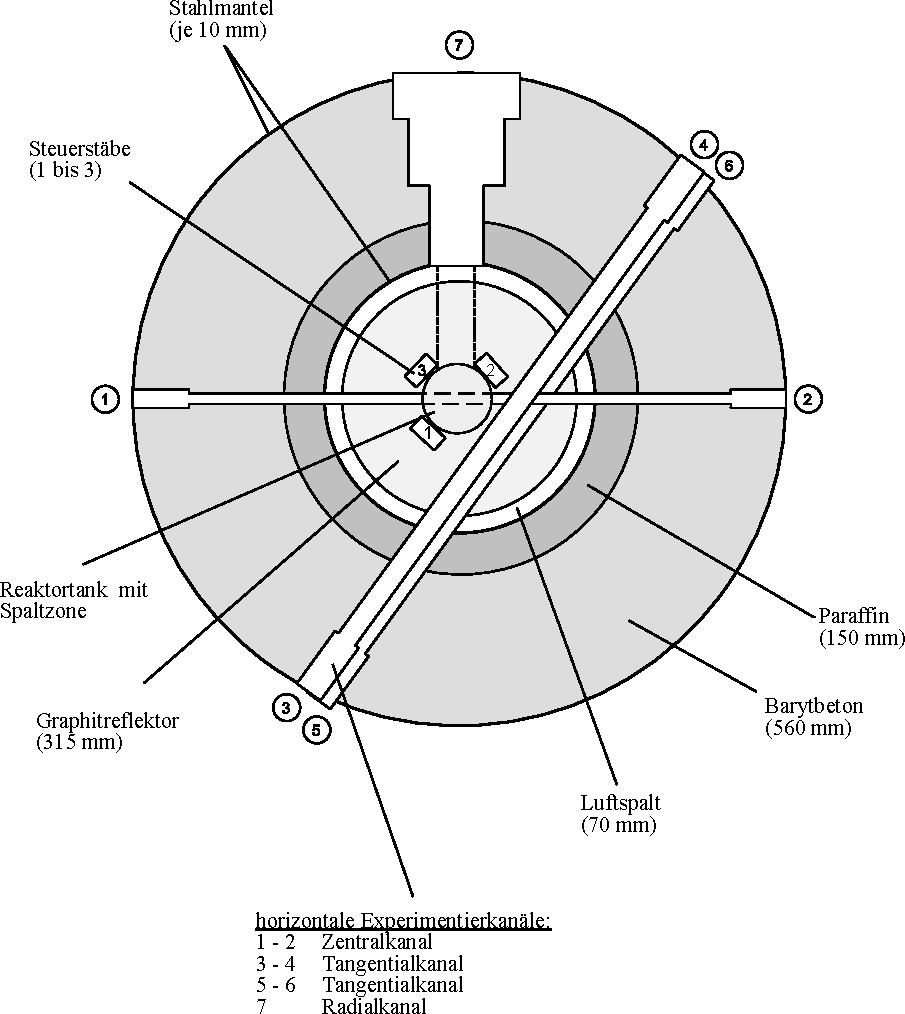
\includegraphics[width=0.7\textwidth]{pic/Horizontalquerschnitt_Reaktor.pdf}
	\caption{Horizontaler Querschnitt, \cite{Aufbau}}
	\label{fig: Horizontaler Querschnitt}
	\end{figure}
	
	\begin{figure}[ht]
	\centering
	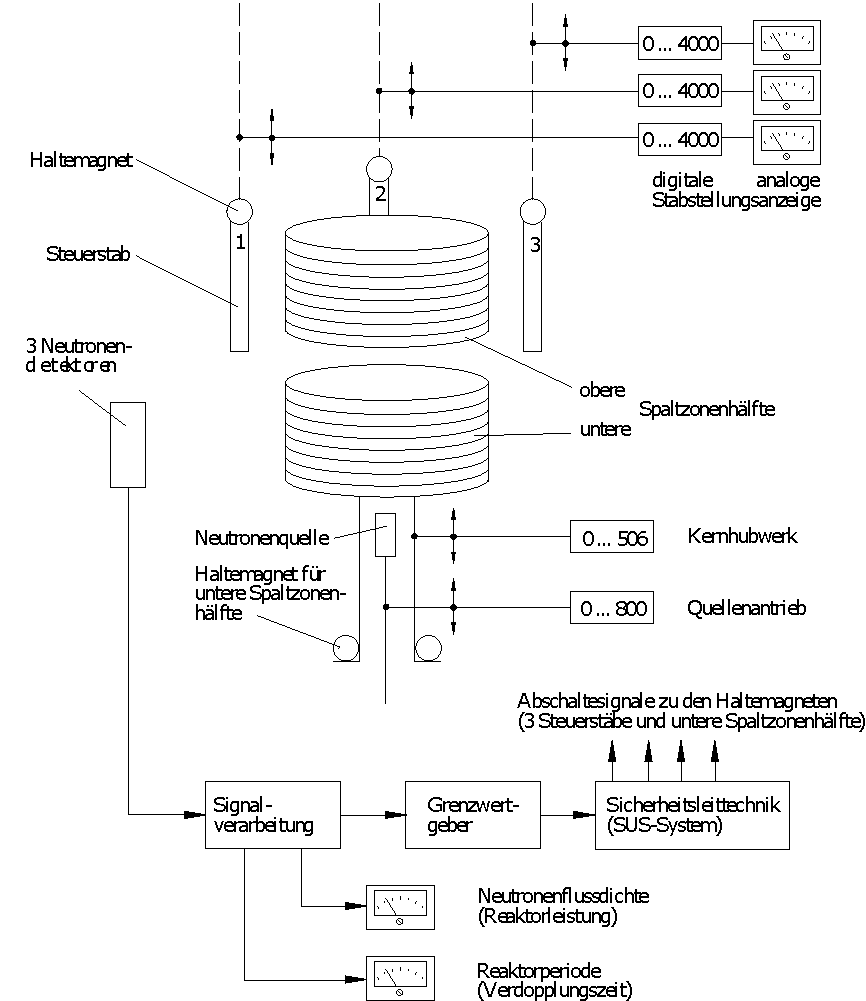
\includegraphics[width=0.6\textwidth]{pic/Reaktoraufbau.pdf}
	\caption{Schematischer Aufbau und Funktionsprinzip, \cite{start} }
	\label{fig: Reaktoraufbau}
	\end{figure}
	
	Eine besondere Bedeutung für die Sicherheit bei der Arbeit mit dem Reaktor spielt das Reaktorschnellabschaltsystem (RESA). Dieses verhindert mittels verschiedener Kontrollmechanismen einen prompt überkritischen Zustand des Reaktors. Dabei existieren die folgenden Grenzwerte:
	\begin{itemize}
	\item Da die \textbf{Reaktorleistung} proportional zur Neutronenflussdichte ist, existiert ein Leistungsgrenzwert von 2,4 W. Diese wird von von drei Neutronenmesskanälen überwacht. Auch wenn die Leistung unter 0,25 W fällt, wird der Reaktor heruntergefahren. Damit wird gewährleistet, dass der Schwellenwert der Auslesegeräte nicht unterschritten wird. Der statistische Fehler ist proportional zu $\frac{1}{\sqrt{N}}$ und würde für N$\rightarrow 0$ gegen unendlich gehen. Diese geringe Leistungsspanne gibt dem AKR den Namen Nulleistungsreaktor.
	\item Die \textbf{Reaktorperiode} darf nicht unter 10 s sinken.
	\item Die \textbf{Temperatur} im Kern darf nicht unter $\unit[18]{^{\circ}C}$ fallen. Bei geringere Temperatur steigt die Dichte des Moderators und damit die Anzahl der für die Kettenreaktion notwendigen thermischen Neutronen.
	\item Auch der \textbf{Unterdruck} darf einen gewissen Wert nicht unterschreiten.
	\item Die Abschaltung des Reaktors erfolgt, sobald im Steuerungssystem oder dem Sicherheitsleitsystem (beispielsweise durch Ausfall der Positionsschalter) eine \textbf{Fehlermeldung} oder ein Ausfall registriert wird.
	\end{itemize}
	
	Tritt die RESA ein, fällt zum einen die untere Kernhälfte zurück in die untere Ausgangslage, zum anderen werden die Cadmium-Steuerstäbe in die unterste Position abgeworfen, indem die Haltemagnete stromlos gemacht werden. Dies senkt sofort massiv die Neutronenflussdichte.\\
	Für einen sicheren Start des Reaktors existiert ein festes Vorgehensschema, wobei die fehlerfreie Funktionsweise der RESA und der Sicherheits- und Steuertechnik bewusst kontrolliert werden. Dafür sind die dazugehörigen Fenster auf dem Bedienungsbildschirm in jeweiliger Farbe gekennzeichnet. Zusätzlich existiert ein Meldungsprotokoll, in dem jeder neue Eintrag bestätigt werden muss, sowie ein Schlüssel zum Zurücksetzen nach dem Eintreten der RESA.
	
	\subsection{Kernspaltung}
	Das Prinzip eines Atomkernreaktors beruht auf einer Kernspaltungskettenreaktion durch Neutronen. Der dafür genutzte Brennstoff Uranoxid ist zu 19,8\% mit U-235 angereichert. Die Halbwertszeit beträgt etwa 704 Millionen Jahre. Durch die Wechselwirkung mit einem Neutron entsteht jedoch kurzzeitig angeregtes U-236, welches in Spaltprodukte zerfällt und dabei zwei oder sogar drei weitere Neutronen entstehen. Auch U-238 kann zu dem instabilen U-239 angeregt werden und als Beginn einer Zerfallskette zu Plutonium umgewandelt werden, was bei Wechselwirkung mit Neutronen auch eine Kettenreaktion auslösen kann. Die dafür notwendigen Startneutronen werden über die natürliche Neutronenquelle $ ^{241} $Americium-Beryllium zugeführt. $ ^{241} $Americium zerfällt unter Aussendung von $\alpha$-Teilchen, welche wiederum mit Beryllium wechselwirken. Als Produkt dieser Wechselwirkung entsteht ein Neutron.\\
	Die zu den Uranisotopen gehörigen Spaltungsquerschnitte sind in Abbildung \ref{fig: Wirkungsquerschnitt_Uran} aufgetragen. Zum einen ist zu erkennen, dass der Wirkungsquerschnitt $\sigma$ von U-239 erst bei wesentlich höheren Neutronenenergien im Vergleich zu U-235 einen nennenswerten Beitrag liefert. Zum anderen wächst $\sigma$ für U-235 für Energien thermischer Neutronen (bei Raumtemperatur $ \simeq \unit[25]{meV} $) um einige Größenordnungen an. Die aus Quelle und Kernspaltung entstehenden schnellen Neutronen besitzen kinetische Energien im MeV Bereich. Für die optimale Nutzung müssen die Neutronen entsprechend abgebremst werden. Dies ist die Aufgabe des Moderators. Gemäß der Impulserhaltung sind für die Abbremsung der Neutronen leichte Atome bzw. Elemente niedriger Ordnungszahl wie Wasserstoff oder Helium geeignet. Auch Feststoffe, die viele Wasserstoffatome enthalten, wie der im AKR verwendete Polyäthylen Kunststoff, werden genutzt.\\
	Unter den entstehenden Neutronen ist zwischen \textbf{prompten} und \textbf{verzögerten} Neutronen zu unterscheiden. Die prompten Neutronen werden direkt bei der Kernspaltung frei gesetzt und besitzen eine Lebensdauer von $\tau = 10^{-4}$s. Ihr Anteil macht im hier verwendeten Uran-235 etwa 99,359$\%$ aus. Die verzögerten Neutronen entstehen andererseits durch den Zerfall von stark angeregten Mutterkernen der Zerfallskette; ihr Einfluss macht sich somit zeitlich verzögert bemerkbar. Darunter lassen sich sechs verschiedene Arten unterscheiden, wobei die zugehörigen Neutronen durch Lebenszeit ($\tau = 0,53...56$s) und Energie charakterisiert sind. Insgesamt machen sie einen Anteil von 0,641 $\%$ an der Neutronenzahl aus.
	
	\begin{figure}[ht]
	\centering
	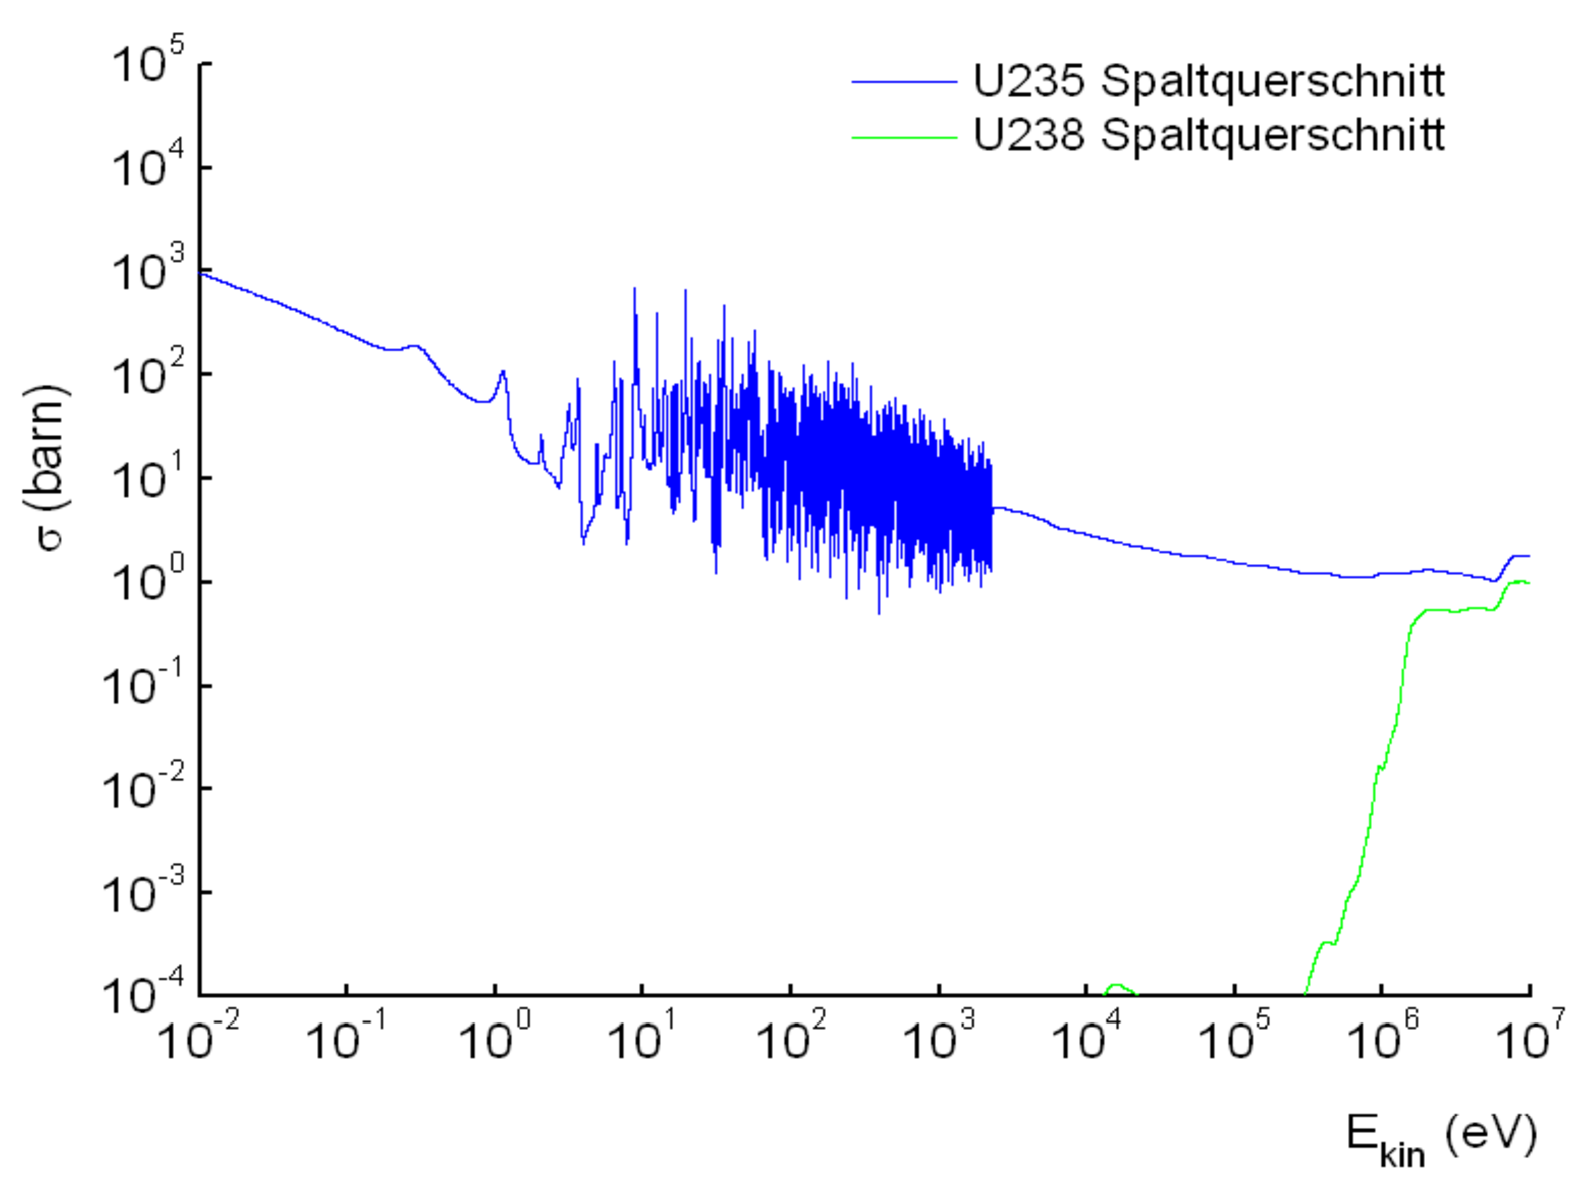
\includegraphics[width=0.8\textwidth]{pic/Wirkungsquerschnitt_Uran.pdf}
	\caption{Doppellogarithmisch aufgetragen sind Spaltungsquerschnitte von U-235 und U-239 in Abhängigkeit der Neutronenenergie,\cite{Wirkungsquerschnitt_Uran}}
	\label{fig: Wirkungsquerschnitt_Uran}
	\end{figure} 
	
	\subsection{Reaktorkinetik}
	
	Die Neutronenflussdichte $\Phi$, $[\Phi]=1 \frac{n}{cm^{2}s}$ stellt im Versuch die zu messende Größe dar. Sie ist proportional zur Reaktorleistung P, $[P] = 1W$, zur Neutronendichte n, $[n= 1 \frac{n}{cm^{3}}]$ und zur Neutronengesamtzahl N.
	Eine Neutronengeneration ist gekennzeichnet durch ihre Lebensdauer l, welche sich ausgehend vom Zeitpunkt der Entstehung zusammensetzt aus Abbremszeit, Diffusionszeit und Reaktionszeit bis zur Bildung eines weiteren Neutrons bei der Kernspaltung.
	Über das Verhältnis der vorhandenen Neutronenzahl zur Zeit t+l zu den Neutronen zur Zeit t lässt sich der Multiplikatorfaktor k berechnen. Er ist ein Maß für die Stärke der Kettenreaktion und definiert den Zustand des Reaktors: 
	\begin{itemize}
	\item k$<$1 unterkritisch
	\item k$=$1 kritisch
	\item k$>$1 überkritisch
	\end{itemize}
	
	
	Um die Veränderung des Zustandes bzw. dessen zeitliches Verhalten zu quantifizieren und einschätzen zu können, werden weitere Größen definiert.
	\begin{itemize}
	\item Die \textbf{Reaktivität $\rho$} mit $\rho=\frac{k-1}{k}$ kann als eine relative Abweichung vom kritischen Zustand betrachtet werden.
	\item Die \textbf{Reaktorperiode T} gibt das Zeitintervall bis zu einer Vergrößerung der Neutronenanzahl um den Faktor $e\approx 2,71$. Entsprechend gilt dies auch für die Leistung P und die Neutronenflussdichte. In der praktischen Umsetzung ist es einfacher die \textbf{Verdopplungszeit T$_{2}$} zu bestimmen. Mittels Formel \ref{eq: Verdopplungszeit_Reaktorperiode} lässt sich diese in die Reaktorperiode überführen.
	\begin{align}
	T&=\frac{T_{2}}{ln2} \label{eq: Verdopplungszeit_Reaktorperiode}
	\end{align}
	
	\item Zusätzlich wird die Größe l$ ^{*} $ mit $l^{*}=\frac{l}{k}$ definiert, welche die mittlere effektive Lebensdauer der Neutronen darstellt.
	\end{itemize}
	
	Im unterkritischen Zustand nähert sich die Neutronendichte n asymptotisch einem Grenzwert n$ _{t=\infty} = \frac{S\cdot l^{*}}{- \rho}$ (S = Quellstärke) an. Die Annäherung an den Grenzwert dauert für größer werdende t umso länger, da sie proportional zu e$ ^{-t} $ erfolgt.\\
	Das Verhalten des Reaktors im überkritschen Zustand wird durch die \textbf{reaktokinetischen Gleichungen} beschrieben:
	\begin{align}
	\frac{dn}{dt}&= \frac{\rho - \beta}{l^{*}}\cdot n + \sum \limits^{6}_{i=1} \lambda_{i}\cdot C_{i} + S\\
	\frac{C_{i}}{dt}&= \frac{\beta _{i}}{l^{*}} \cdot n - \lambda _{i} \cdot C_{i}
	& \text{i= 1, ... , 6}
	\end{align}
	
	Dieses Gleichungssystem aus 7 Differentialgleichungen wird vereinfacht, indem die unterschiedlichen Anteile $\beta _{i}$ an verzögerten Neutronen der 6 Mutterkerngruppen zu einem Mittelwert zusammengefasst werden.
	
	\begin{align}
	\beta= \sum \limits^{6}_{i=1} \beta _{i} &\Rightarrow \frac{1}{\lambda} = \frac{1}{\beta} \sum \limits^{6}_{i=1} \frac{\beta_{i}}{\lambda _{i}}
	\end{align}
	
	Man erhält ein Gleichungssystem aus zwei gekoppelten Differentialgleichungen:
	
	\begin{align}
	\frac{dn}{dt}&= \frac{\rho - \beta}{l^{*}} \cdot n + \lambda \cdot C + S\\
	\frac{C}{dt}&= \frac{\beta}{l^{*}} \cdot n - \lambda \cdot C
	\end{align}
	
	Unter der Annahme einer sprunghaften Reaktivitätsänderung $\rho = 0, t<0$ und $\rho = const, t\geq 0$ und Vernachlässigung der Quellneutronen S ergibt sich als Lösung der Neutronendichte
	\begin{align}
	n(t)&= n_{0} \left[ \frac{\beta}{\beta - \rho} e^{\frac{\lambda \cdot \rho}{\beta - \rho}\cdot t} - \frac{\rho}{\beta - \rho} e^{-\frac{\beta - \rho}{l^{*}} \cdot t} \right] \label{eq: Lösung_kinGlg}
	\end{align}
	
	Die beiden Terme sind von verschiedener Bedeutung für den Reaktorzustand.
	\begin{itemize}
	\item Für den \textbf{verzögerten überkritischen Reaktor $\rho < \beta$} fällt der zweite Term auf Grund von l$ ^{*} = 10^{-4}$ s in wenigen Sekunden ab. Der übrig bleibende Term charakterisiert die Veränderung der Neutronendichte, indem nach einer plötzlichen Reaktivitätserhöhung ein durch die prompten Neutronen verursachter und entsprechend benannter prompter Sprung erfolgt. Für einen weiteren Anstieg sorgt der Einfluss der verzögerten Neutronen, für die der Reaktor überkritisch wird. Nach einer gewissen Zeit stellt sich die \textbf{stabile Reaktorperiode T$ _{S}$} ein. Die Einstellzeit entsteht durch die verschiedenen Neutronengruppen und die entsprechend unterschiedlichen Lebensdauern. Der zweite Exponentialterm fällt unterschiedlich schnell ab.
	\item Für den Fall des \textbf{prompt überkritischen Reaktors $\rho > \beta$} wird der Exponent des zweiten Terms der Formel \ref{eq: Lösung_kinGlg} positiv. Der Reaktor wird mit einer Reaktorperiode im Millisekundenbereich durch prompten Neutronen allein überkritisch. Dieser Zustand ist mit den Steuerstäben nicht mehr kontrollierbar und ist unbedingt zu vermeiden.
	\end{itemize}
	
	Wird beim Einstellen des Reaktorzustandes nun die Reaktivität um ein definiertes Stück verändert (beispielsweise durch Positionsänderung der Steuerungsstäbe oder Einführung einer Probe), äußert sich dies im Leistungsverhalten wie in Abb. \ref{fig: leistungsverhalten} für $\Delta \rho >0$ für den überkritischen Reaktor dargestellt. Der überkritische Zustand ist, wie beschrieben, am exponentiellen Anstieg der Neutronendichte nach etwa 100 s zu erkennen. Wird der kritische Zustand erreicht, bleibt die Neutronendichte konstant, für den unterkritischen Zustand fällt sie exponentiell ab. Gut zu erkennen ist der prompte Sprung in positive Richtung, welcher nach jeder positiven Reaktivitätsänderung - unabhängig des Reaktorzustandes - auftritt. Umgekehrt erfolgt der Sprung in negative Richtung für $\Delta \rho <0$. Dazu kommt das analoge Verhalten der verzögerten Reaktion. Dieser Effekt fordert bei der Einstellung des Reaktorzustandes die entsprechende Wartezeit, bis sich T$_{S}$ eingestellt hat, um das weitere Vorgehen zu prüfen.
	
	\begin{figure}[ht]
	\centering
	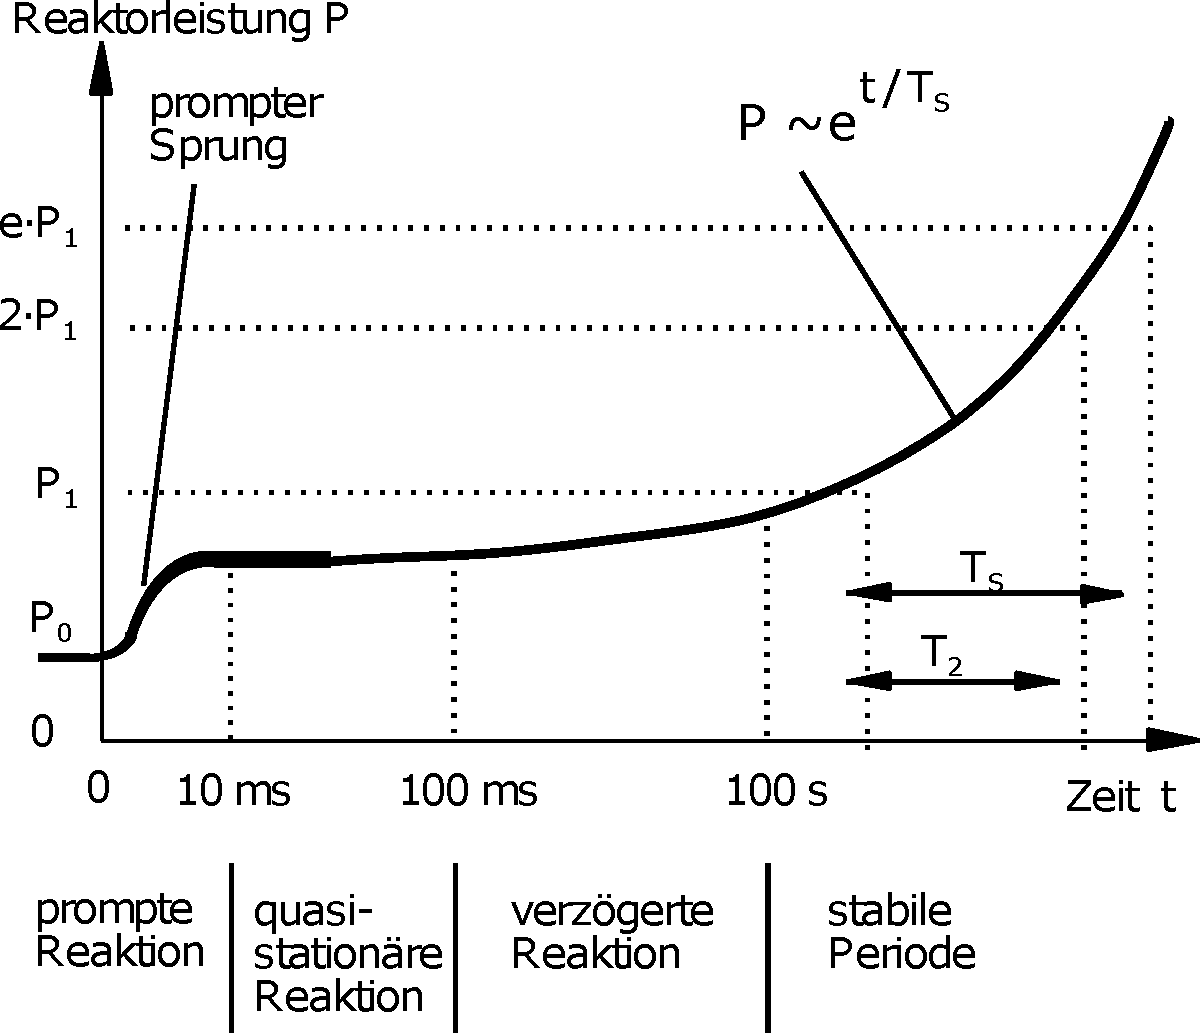
\includegraphics[width=0.8\textwidth]{pic/Leistungsaenderung.pdf}
	\caption{Leistungszeitsverhalten bei plötzlicher definierter, positiver Reaktivitätsänderung, \cite{start}}
	\label{fig: leistungsverhalten}
	\end{figure}
	
	\subsection{Steuerstabkalibrierung}
	%TODO: Gleichung für differentielle / integrale Steuerstabkennlinie, INHOUR-Gleichung, Gesamt-, Überschuss-, Abschaltreaktivität.
	Um die nukleare Sicherheit eines Kernreaktors jederzeit gewährleisten zu können, ist es wichtig, dass man weiß, wie sich die Neutronenbilanz im Reaktor unter Veränderung der vorhandenen Steuer- und Regeleinrichtungen verhält. Zu diesem Zweck bestimmt man die \textit{differentiellen} und \textit{integralen Steuerstabkennlinien} der vorliegenden Neutronenabsorber. \\
	Da die axiale Neutronenflussdichte $\Phi_z(z)$ eines zylindersymmetrischen Reaktors zum Rand der Spaltzone abnimmt, wird ein Steuerstab, der sich in der Mitte bewegt einen größeren Einfluss auf die Reaktivität haben als ein sich am Rand bewegender. Eine durch diesen Effekt erzeugte Reaktivitätsveränderung $\mathrm{d}\rho$ ist also proportional zur Neutronenflussdichte $\Phi_z(z)$, der Absorptionswahrscheinlichkeit der Neutronen am Absorber (Wechselwirkungsquerschnitt) $\Sigma_a$ und der eingeschobenen Länge $\mathrm{d}z$. Abbildung \ref{int:NeutrFlDichte} zeigt die ortsabhängige Neutronenflussdichteverteilung in der Spaltzone.\\
		\begin{figure}[ht]
			\centering
			\captionsetup{justification=centering}
			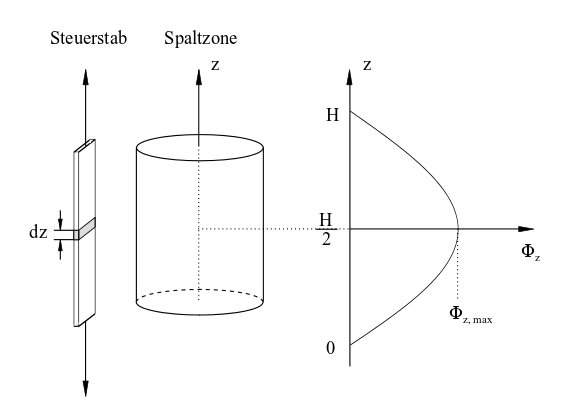
\includegraphics[scale=0.4]{pic/NeutrFlDichte}
			\caption{Zylindrische Spaltzone mit ortsabhängiger Neutronenflussdichte $\Phi_z(z)$\cite{stab}}
			\label{int:NeutrFlDichte}
		\end{figure}
	\ \\
	Da Neutronen auch durch Oberflächenverluste ohne Absorption verloren gehen können, definiert man eine sogenannte \textit{Einflussfunktion} $f(z)$ , die beschreibt, wie groß der Einfluss der Neutronen am Ort $z$ auf die Reaktivität ist. Neutronen am Rand haben durch ihre höhere Verlustwahrscheinlichkeit einen geringeren Einfluss, weshalb die Einflussfunktion in etwa proptional zur Neutronendichte (welche zum Rand hin auch abnimmt) sein muss, d.h. $f(z) \propto \Phi_z(z)$. Überlagern wir diese beiden statistisch unabhängigen Effekte erhalten wir die \textit{differentielle Steuerstabkennlinie}:\\
	$$\frac{\mathrm{d}\rho}{\mathrm{d}z}(z) \propto \Sigma_a \cdot \Phi_z(z)$$
	Integrieren wir diese über eine makroskopische Länge z und normieren diese anschließend auf den Maximalwert $\rho_{max}$, erhalten wir die \textit{integrale Steuerstabkennlinie}:
	$$\frac{\rho(z)}{\rho_{max}} = \frac{z}{H} - \frac{1}{2\pi} \sin{\left(\frac{2\pi z}{H}\right)}$$
	Wobei H die effektive Länge der Spaltzone beschreibt. Abbildung zeigt den typischen Verlauf der Steuerstabkennlinien:
		\begin{figure}[ht]
				\centering
				\captionsetup{justification=centering}
				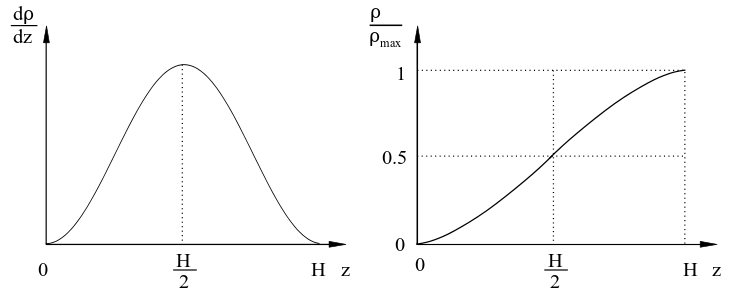
\includegraphics[scale=0.4]{pic/sskl}
				\caption{links: differentielle Steuerstabkennlinie, 
						\\rechts: integrale, auf Maximalwert normierte Steuerstabkennlinie\cite{stab}}
				\label{int:NeutrFlDichte}
		\end{figure}
	\ \\
	Im Versuch wird die Reaktivität über die Messung der stabilen Reaktorperiode $T_s$ beziehungsweise der Verdopplungszeit $T_2$ angewandt, d.h. man misst die Zeit, in der sich die Reaktorleistung verdoppelt. Die Lösung für die Neutronendichte $n(t)$ der reaktorkinetischen Gleichungen ist exakterweise eine Linearkombination von 7 Termen $\propto e^{\omega_i t}$. Da sechs dieser Terme bei positiver Reaktivitätsänderung einen negativen Exponenten besitzen, klingen diese nach einer gewissen Zeit ab. Verändert man also die Stabposition des kritischen Reaktors so, dass er überkritisch wird, muss erst eine Weile gewartetet werden, bevor man die Reaktorperiode messen kann. Dies muss bei der Messung später beachtet werden, da sonst die unter dieser Annahme hergeleitete \textit{Inhour-Gleichung} (\ref{int:inhour}) nicht gilt:
	\begin{equation}\label{int:inhour}
		\rho\prime = \frac{\rho}{\beta} = \frac{l^*/\beta }{T_s}+ \sum_{i=1}^{6} \frac{a_i}{1 + \lambda_i\cdot T_s}
	\end{equation}
	Hierbei sind:\\
	$l^*$...mittlere Lebensdauer der promten Neutronen\\
	$\beta_i$...absoluter Anteil der verzögerten Neutronen der i-ten Gruppe\\
	$\lambda_i$...Zerfallskonstante der Mutterkerne der i-ten Gruppe\\
	Am AKR gilt: $l^* / \beta = 0,0051\ \unit{s}$. Abbildung \ref{int:datenInhour} fasst die verwendeten Parameter zusammen:
		\begin{figure}[ht]
					\centering
					\captionsetup{justification=centering}
					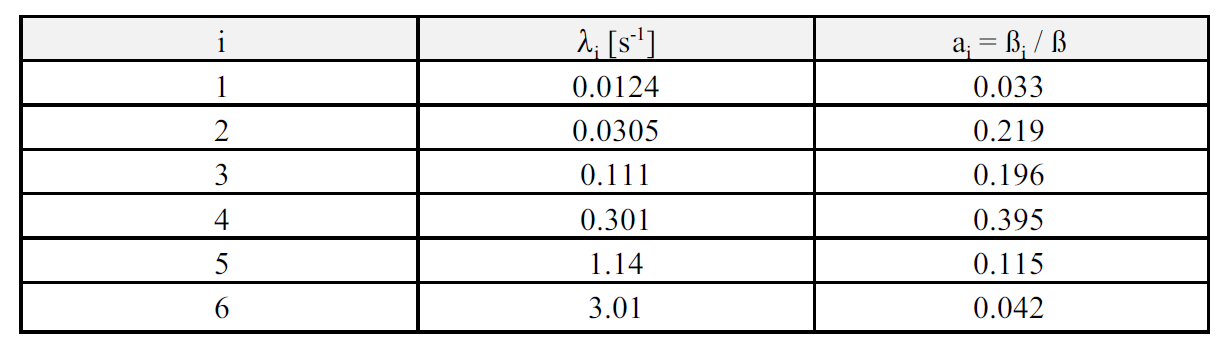
\includegraphics[scale=0.3]{pic/daten_inhour}
					\caption{Daten für die Mutterkerne der verzögerten Neutronen in der Inhour-Gleichung\cite{stab}}
					\label{int:datenInhour}
		\end{figure}
	\ \\
	In der Praxis ist es wichtig zu wissen, welchen Einfluss ein einzelner Steuerstab auf die Reaktivität hat. Dafür definiert man die folgenden Größen:
		\begin{itemize}
			\item \textit{Gesamtreaktivität} $\rho_{ges}$ ist die zugeführte Reaktivität über die gesamte Hubhöhe
			\item \textit{Überschussreaktivität} $\rho_{\ddot{U}berschuss}$ ist diejenige positive Reaktivität, die ausgehend vom kritischen Zustand des Reaktors durch Heben aller Steuerstäbe in die obere Endlage zugeführt werden kann. Ist diese Größe kleiner als $1\ \unit{\$}$ kann weder durch technische noch Bedienfehler ein prompt überkritischer Reaktorzustand erreicht werden. Man liest diese in der integralen Steuerstabkennlinie ab, indem man ausgehend von einem beliebigen kritischen Zustand den Abstand der Kurve zur Gesamtreaktivität eines einzelnen Stabes betrachtet. Die gesamte Überschussreaktivität ist dann die Summe aus denen der Einzelstäbe. Abbildung \ref{int:ueberschuss} verdeutlicht dies.
			\item \textit{Abschaltreaktivität} $\rho_{Abschalt}$ ist dann der negative Reaktivitätswert, der ausgehend vom kritischen Zustand des Reaktors durch Abfallen aller Steuerstäbe in die Spaltzone zugeführt wird. Es gilt $\rho_{Abschalt} = \rho_{ges} - \rho_{\ddot{U}berschuss}$. 
		\end{itemize}
		\begin{figure}[ht]
							\centering
							\captionsetup{justification=centering}
							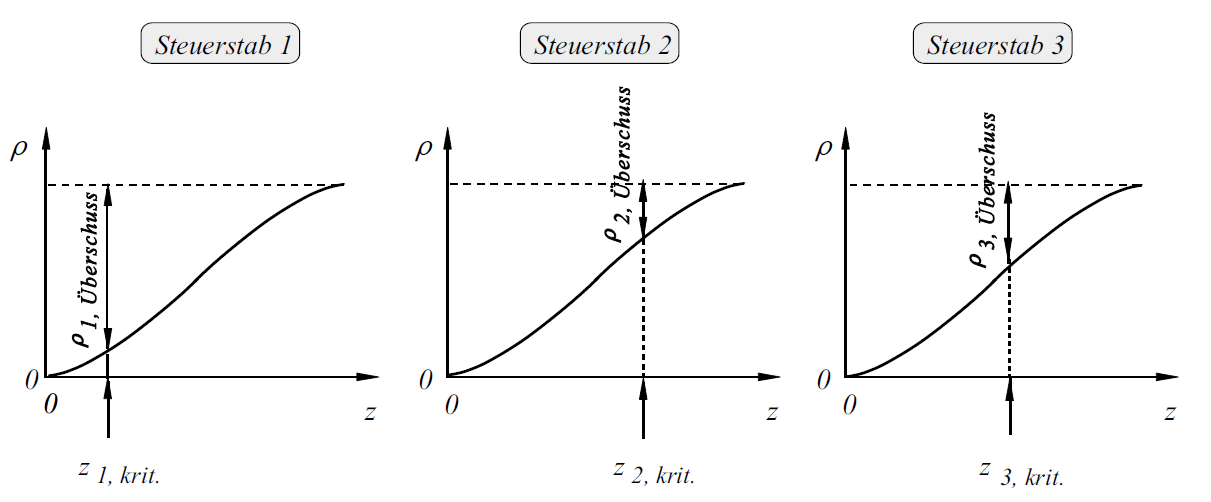
\includegraphics[scale=0.3]{pic/ueberschuss}
							\caption{Bestimmung der Überschussreaktivität aus den integralen Steuerstabkennlinien\cite{stab}}
							\label{int:ueberschuss}
		\end{figure}
	